
%% bare_conf.tex
%% V1.4b
%% 2015/08/26
%% by Michael Shell
%% See:
%% http://www.michaelshell.org/
%% for current contact information.
%%
%% This is a skeleton file demonstrating the use of IEEEtran.cls
%% (requires IEEEtran.cls version 1.8b or later) with an IEEE
%% conference paper.
%%
%% Support sites:
%% http://www.michaelshell.org/tex/ieeetran/
%% http://www.ctan.org/pkg/ieeetran
%% and
%% http://www.ieee.org/

%%*************************************************************************
%% Legal Notice:
%% This code is offered as-is without any warranty either expressed or
%% implied; without even the implied warranty of MERCHANTABILITY or
%% FITNESS FOR A PARTICULAR PURPOSE! 
%% User assumes all risk.
%% In no event shall the IEEE or any contributor to this code be liable for
%% any damages or losses, including, but not limited to, incidental,
%% consequential, or any other damages, resulting from the use or misuse
%% of any information contained here.
%%
%% All comments are the opinions of their respective authors and are not
%% necessarily endorsed by the IEEE.
%%
%% This work is distributed under the LaTeX Project Public License (LPPL)
%% ( http://www.latex-project.org/ ) version 1.3, and may be freely used,
%% distributed and modified. A copy of the LPPL, version 1.3, is included
%% in the base LaTeX documentation of all distributions of LaTeX released
%% 2003/12/01 or later.
%% Retain all contribution notices and credits.
%% ** Modified files should be clearly indicated as such, including  **
%% ** renaming them and changing author support contact information. **
%%*************************************************************************



\documentclass[a4paper, conference]{IEEEtran}


%\usepackage{epstopdf}

\ifCLASSINFOpdf
  \usepackage[pdftex]{graphicx}
\else
\fi
% graphicx was written by David Carlisle and Sebastian Rahtz. It is
% required if you want graphics, photos, etc. graphicx.sty is already
% installed on most LaTeX systems. The latest version and documentation
% can be obtained at: 
% http://www.ctan.org/pkg/graphicx
% Another good source of documentation is "Using Imported Graphics in
% LaTeX2e" by Keith Reckdahl which can be found at:
% http://www.ctan.org/pkg/epslatex
%
% latex, and pdflatex in dvi mode, support graphics in encapsulated
% postscript (.eps) format. pdflatex in pdf mode supports graphics
% in .pdf, .jpeg, .png and .mps (metapost) formats. Users should ensure
% that all non-photo figures use a vector format (.eps, .pdf, .mps) and
% not a bitmapped formats (.jpeg, .png). The IEEE frowns on bitmapped formats
% which can result in "jaggedy"/blurry rendering of lines and letters as
% well as large increases in file sizes.
%
% You can find documentation about the pdfTeX application at:
% http://www.tug.org/applications/pdftex





% *** MATH PACKAGES ***
%
%\usepackage{amsmath}
% A popular package from the American Mathematical Society that provides
% many useful and powerful commands for dealing with mathematics.
%
% Note that the amsmath package sets \interdisplaylinepenalty to 10000
% thus preventing page breaks from occurring within multiline equations. Use:
%\interdisplaylinepenalty=2500
% after loading amsmath to restore such page breaks as IEEEtran.cls normally
% does. amsmath.sty is already installed on most LaTeX systems. The latest
% version and documentation can be obtained at:
% http://www.ctan.org/pkg/amsmath





% *** SPECIALIZED LIST PACKAGES ***
%
%\usepackage{algorithmic}
% algorithmic.sty was written by Peter Williams and Rogerio Brito.
% This package provides an algorithmic environment fo describing algorithms.
% You can use the algorithmic environment in-text or within a figure
% environment to provide for a floating algorithm. Do NOT use the algorithm
% floating environment provided by algorithm.sty (by the same authors) or
% algorithm2e.sty (by Christophe Fiorio) as the IEEE does not use dedicated
% algorithm float types and packages that provide these will not provide
% correct IEEE style captions. The latest version and documentation of
% algorithmic.sty can be obtained at:
% http://www.ctan.org/pkg/algorithms
% Also of interest may be the (relatively newer and more customizable)
% algorithmicx.sty package by Szasz Janos:
% http://www.ctan.org/pkg/algorithmicx




% *** ALIGNMENT PACKAGES ***
%
%\usepackage{array}
% Frank Mittelbach's and David Carlisle's array.sty patches and improves
% the standard LaTeX2e array and tabular environments to provide better
% appearance and additional user controls. As the default LaTeX2e table
% generation code is lacking to the point of almost being broken with
% respect to the quality of the end results, all users are strongly
% advised to use an enhanced (at the very least that provided by array.sty)
% set of table tools. array.sty is already installed on most systems. The
% latest version and documentation can be obtained at:
% http://www.ctan.org/pkg/array


% IEEEtran contains the IEEEeqnarray family of commands that can be used to
% generate multiline equations as well as matrices, tables, etc., of high
% quality.




% *** SUBFIGURE PACKAGES ***
%\ifCLASSOPTIONcompsoc
%  \usepackage[caption=false,font=normalsize,labelfont=sf,textfont=sf]{subfig}
%\else
%  \usepackage[caption=false,font=footnotesize]{subfig}
%\fi
% subfig.sty, written by Steven Douglas Cochran, is the modern replacement
% for subfigure.sty, the latter of which is no longer maintained and is
% incompatible with some LaTeX packages including fixltx2e. However,
% subfig.sty requires and automatically loads Axel Sommerfeldt's caption.sty
% which will override IEEEtran.cls' handling of captions and this will result
% in non-IEEE style figure/table captions. To prevent this problem, be sure
% and invoke subfig.sty's "caption=false" package option (available since
% subfig.sty version 1.3, 2005/06/28) as this is will preserve IEEEtran.cls
% handling of captions.
% Note that the Computer Society format requires a larger sans serif font
% than the serif footnote size font used in traditional IEEE formatting
% and thus the need to invoke different subfig.sty package options depending
% on whether compsoc mode has been enabled.
%
% The latest version and documentation of subfig.sty can be obtained at:
% http://www.ctan.org/pkg/subfig




% *** FLOAT PACKAGES ***
%
%\usepackage{fixltx2e}
% fixltx2e, the successor to the earlier fix2col.sty, was written by
% Frank Mittelbach and David Carlisle. This package corrects a few problems
% in the LaTeX2e kernel, the most notable of which is that in current
% LaTeX2e releases, the ordering of single and double column floats is not
% guaranteed to be preserved. Thus, an unpatched LaTeX2e can allow a
% single column figure to be placed prior to an earlier double column
% figure.
% Be aware that LaTeX2e kernels dated 2015 and later have fixltx2e.sty's
% corrections already built into the system in which case a warning will
% be issued if an attempt is made to load fixltx2e.sty as it is no longer
% needed.
% The latest version and documentation can be found at:
% http://www.ctan.org/pkg/fixltx2e


%\usepackage{stfloats}
% stfloats.sty was written by Sigitas Tolusis. This package gives LaTeX2e
% the ability to do double column floats at the bottom of the page as well
% as the top. (e.g., "\begin{figure*}[!b]" is not normally possible in
% LaTeX2e). It also provides a command:
%\fnbelowfloat
% to enable the placement of footnotes below bottom floats (the standard
% LaTeX2e kernel puts them above bottom floats). This is an invasive package
% which rewrites many portions of the LaTeX2e float routines. It may not work
% with other packages that modify the LaTeX2e float routines. The latest
% version and documentation can be obtained at:
% http://www.ctan.org/pkg/stfloats
% Do not use the stfloats baselinefloat ability as the IEEE does not allow
% \baselineskip to stretch. Authors submitting work to the IEEE should note
% that the IEEE rarely uses double column equations and that authors should try
% to avoid such use. Do not be tempted to use the cuted.sty or midfloat.sty
% packages (also by Sigitas Tolusis) as the IEEE does not format its papers in
% such ways.
% Do not attempt to use stfloats with fixltx2e as they are incompatible.
% Instead, use Morten Hogholm'a dblfloatfix which combines the features
% of both fixltx2e and stfloats:
%
% \usepackage{dblfloatfix}
% The latest version can be found at:
% http://www.ctan.org/pkg/dblfloatfix




% *** PDF, URL AND HYPERLINK PACKAGES ***
%
\usepackage{url}
% url.sty was written by Donald Arseneau. It provides better support for
% handling and breaking URLs. url.sty is already installed on most LaTeX
% systems. The latest version and documentation can be obtained at:
% http://www.ctan.org/pkg/url
% Basically, \url{my_url_here}.




% *** Do not adjust lengths that control margins, column widths, etc. ***
% *** Do not use packages that alter fonts (such as pslatex).         ***
% There should be no need to do such things with IEEEtran.cls V1.6 and later.
% (Unless specifically asked to do so by the journal or conference you plan
% to submit to, of course. )


% correct bad hyphenation here
\hyphenation{op-tical net-works semi-conduc-tor}

%\epstopdfsetup{outdir=./img}

\begin{document}
%
% paper title
% Titles are generally capitalized except for words such as a, an, and, as,
% at, but, by, for, in, nor, of, on, or, the, to and up, which are usually
% not capitalized unless they are the first or last word of the title.
% Linebreaks \\ can be used within to get better formatting as desired.
% Do not put math or special symbols in the title.
\title{OPQ Version 2: An Architecture for Distributed, Real-Time, High Performance Power Data Acquisition, Analysis, and Visualization}


\author{\IEEEauthorblockN{Anthony J. Christe, Sergey I. Negrashov, Philip M. Johnson, Dylan Nakahodo, David Badke, David Aghalarpour}
\IEEEauthorblockA{
    Collaborative Software Development Lab\\
    Department of Information and Computer Sciences\\
University of Hawaii at Manoa
}}


% make the title area
\maketitle

% As a general rule, do not put math, special symbols or citations
% in the abstract
\begin{abstract}
OpenPowerQuality (OPQ) is a framework that supports end-to-end capture, analysis, and visualizations of distributed real-time power quality (PQ) data. Version 2 of OPQ builds on version 1 by providing higher sampling rates, optional battery backup, end-to-end security, GPS synchronization, pluggable analysis, and a real-time visualization framework. OPQ provides real-time distributed power measurements which allows users to see both local PQ events and grid-wide PQ events. The OPQ project has three principal components: back-end hardware for making power measurements, middleware for data acquisition and analysis, and a front-end providing visualizations. OPQBox2 is a hardware platform that takes PQ measurements, provides onboard analysis, and securely transfers data to our middleware. The OPQ middleware performs filtering on the OPQBox2 sensor data and performs high-level PQ analysis. The results of our PQ analysis and real-time state of the sensor network are displayed using OPQView. We've collected distributed PQ data from locations across Oahu, Hawaii and have demonstrated our ability to detect both local and grid-wide power quality events.
\end{abstract}
\IEEEpeerreviewmaketitle

\section{Introduction}
As power grids transition from a centralized generation model to a distributed model, maintaining stability requires fine grained knowledge of the grid's state\cite{ECPAB}. Monitoring power quality (PQ) on a distributed generation smartgrid requires a distributed sensor network. How do we collect, analyze, and visualize PQ at the power grid scale using data gathered from residential utility customers? 

To answer this question, we developed and deployed an open source hardware and software system focused on consumer level monitoring across Oahu called Open Power Quality (OPQ). Version 2 of OPQ (OPQ2) is able to aggregate distributed PQ measurements, perform high level real-time PQ analysis and classification, and display PQ at both the consumer and grid level. OPQ2 is a multi-layered framework consisting of custom hardware for collecting distributed PQ data (OPQBox2), a middleware for filtering and event detection (OPQMakai), higher level PQ analysis (OPQMauka), and finally a front-end for consumer friendly grid level PQ visualizations (OPQView). The OPQ2 architecture is shown in figure \ref{fig:system-architecture}.

%In late 2014 we performed a pilot study to test the feasibility of our hardware and software system. Data collected during this study showed strong correlations between PV production and daily voltage trends. We demonstrated that a grid wide view allows us to determine if PQ events take place at the consumer level or at the grid level. 

Each OPQBox2 processes 2.7 billion samples per day. Using node level feature extraction, OPQBox2's forwards only 500,000 measurements to the cloud service in the same 24 hours. Further analysis and filtering yields roughly 1 distributed PQ event per day. These events contain data from every device on the network sampled at full resolution and sampling rate.  Through the use of our multi-tiered system, we aim to bring grid operators and end users, useful, intuitive, actionable, real-time information about the power grid.

%Finally, we could produce these boxes for under \$100 each. This is roughly an order of magnitude cheaper than other power quality monitoring equipment and is better suited for our applications.

\begin{figure*}[htb!]\label{fig:system-architecture}
    \centering
    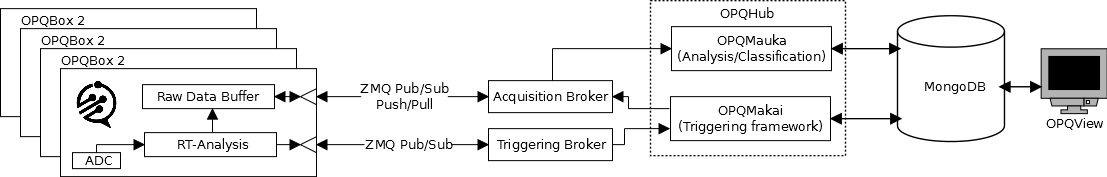
\includegraphics[width=0.9\linewidth]{img/system-diagram}
    \caption{OPQ System Architecture}
\end{figure*}

\section{OPQ Version 2 Architecture}
\subsection{OPQBox2}
OPQBox2 is a modern, high performance, power quality monitor built with distributed measurements in mind. OPQBox2 provides high resolution sampled data of up to 50kS/s at 16bits. Optional GPS synchronization and battery backup can be added to the OPQBox2 to tailor it to a specific power quality measurement. 

While sampling and GPS synchronization is controlled by the realtime DSP, all of the signal processing and communication is controlled by a Raspberry PI single board computer. The Raspberry PI collects 10 AC cycles of ADC measurements at a time and computes the utility frequency and $V_{rms}$. These values are sent to the cloud triggering broker via WiFi while the raw waveforms are buffered in the local Redis key value store.

%Each chunk is stored is a Redis sorted-set, indexed by timestamp. Range queries on raw waveform data occur in $\mathcal{O}(\log{}n + m)$ time. Older entries in the buffer are expired via a garbage collection process after a configurable amount of time. 

If the triggering data stream indicates a power quality event, our middleware may request raw waveforms from the affected OPQBox2s. When the triggering server requests data from an OpqBox2, it requests a time range. This data is queried from Redis, serialized into a single large data packet, and transferred back to the requesting server. All of the communication between the OPQBox2 and the cloud services are done over an encrypted ZeroMQ connection\cite{fengping2012distributed}.

Time synchronization of the OPQBox2 is performed via Network Time Protocol (NTP)\cite{mills1991internet}. While OPQBox2's are able to synchronize via GPS, we found NTP to be suitable for our system. We have verified the synchronization provided by Network Time Protocol (NTP) by comparing frequency measurements collected from two OPQBox2 devices and examining their phase difference.

%We also confirm the frequency resolution of the OPQBox by supplying it a 60 Hz signal from a function generator and observing the data recorded by the box. We plot the frequency data and found that our box can accurately record the frequency supplied by the generator.

\subsection{OPQHub}
OPQHub is OPQ's middleware system and is responsible for collecting raw and feature extracted data from OPQBox2's and for performing high level PQ analysis.  OPQHub is split into two components, OPQMakai, a pluggable filtering and data request component and OPQMauka, a pluggable real-time PQ analysis component.

All communication between the OPQBox2 and OPQHub passes through two connection brokers. These brokers allow us to terminate encryption at the cloud boundary, thus simplifying the analysis framework. ZeroMQ is used throughout our cloud infrastructure to connect the analysis plugins to brokers and other plugins. This allows us to form ad-hoc analysis topologies, such pipeline processing, and map reduce pipelines without interfering with regular data acquisition.

The triggering stream consists of the feature reduced data(frequency and $V_{rms}$) for each device in the OPQ2 network. This stream is brokered via the triggering broker, and analyzed by the set of analysis plugins called OPQMakai. If multiple devices show temporally coherent deviation from the norm, OPQMakai will request the raw data from OPQBox2 devices via the acquisition broker. 

Further analysis of the raw waveform is performed by  the OPQMauka analysis and classification system. Each of the plugins in OPQMauka are responsible for different PQ classification and analysis tasks. We currently implement plugins that detect and report PQ measurements, voltage sags and swells, frequency sags and swells, and perform ITIC event classification of voltage events. We've also developed plugins that, along with the filtering framework OPQMakai, allow us to detect these events on a distributed level. Data products from OPQMauka are stored in MongoDB and presented to clients use OPQView.


%For example, the voltage analysis plugin will monitor voltage thresholds and report voltage dips and swells. When the voltage plugin encounters an event, it will produce a voltage event message. The ITIC plugin will consume voltage event messages and classify them by their ITIC classification.


\subsection{OPQView}
OPQView serves as the front-end user interface of the OPQ2 system. It is implemented in JavaScript using MeteorJS. OPQView serves as the end-point of OPQ2. OPQView is responsible for displaying collected PQ data in a useful and meaningful way. OPQView maintains a communications interface with OPQHub via a MongoDB database, from which it is able to reactively retrieve real-time PQ data. This data includes voltages and frequencies measured by individual devices, as well as PQ events and their corresponding waveforms.  OPQView does not only serve as a front-end to display real-time data, but it can also display historical grid trends and power quality events. 
%Over time, OPQHub aims to determine patterns in these distributed events, which would allow OPQView to determine 'communities' of devices with similar PQ characteristics. 

The real-time nature of our data allows for a wide potential of visualization techniques - such as real-time heat maps of device voltages and frequencies across the grid. OPQView also supplies the administrative interface for OPQBox2's, allowing device owners to adjust their device's privacy and sharing settings as needed. 

\begin{figure}[h]
    \centering
    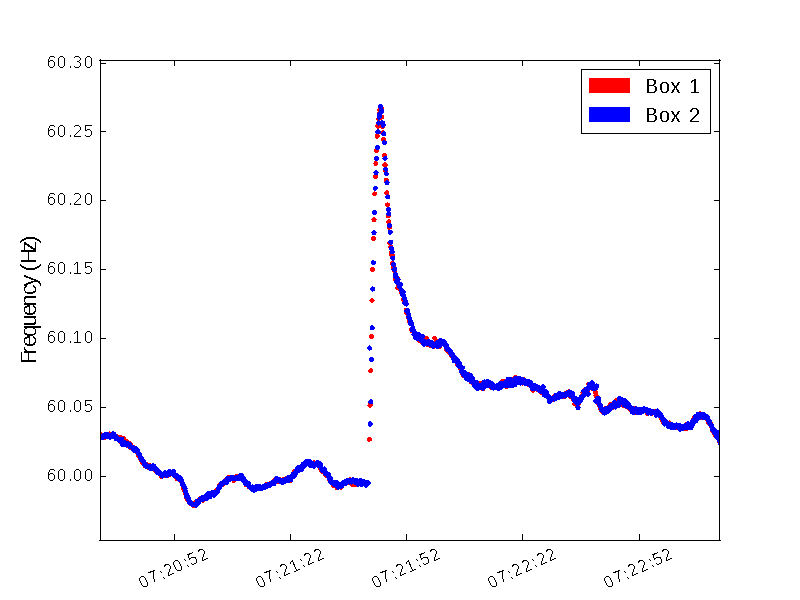
\includegraphics[width=0.9\columnwidth]{img/Event1_f.png}
    \caption{Frequency event. March 1st 2017.}
    \label{fig:event}
\end{figure}

\section{Results}

Currently, OPQHub is capable of detecting and recording frequency and 
voltage based PQ events. Voltage based events include sags, swells.
Frequency events are limited to frequency deviation from the 60Hz nominal. Example of a triggering stream of a frequency event is shown in Figure \ref{fig:event}. This event occurred during the lighting storm March 1st 2017, and is likely a lighting strike. Two devices were separated by 5 miles and were connected to different substations. 
%While utility voltage varies wildly between households, utility frequency tends to track closely across the entire grid. 

Frequency deviations on the order of $\frac{1}{4}$Hz, can lead to load shedding\cite{GE_LS}. This is a process where a section of the power grid is disconnected from the utility in order to preserve grid stability. Collection and analysis of events such as this one will ultimately lead to insights into power grid operation, and give utility customers a more active role in power grid monitoring.

%\section{Conclusion}
%We designed a low cost, real-time, open-source framework capable of aggregating distributed PQ measurements, requesting raw PQ data from specific devices, performing high level real-time PQ analysis and classification, and displaying PQ at both the consumer level and the grid level. 
%
%Our system detected multiple local and grid-level PQ events and can also display the current real-time state of the power grid. [TODO: Finish conclusion]

% can use a bibliography generated by BibTeX as a .bbl file
% BibTeX documentation can be easily obtained at:
% http://mirror.ctan.org/biblio/bibtex/contrib/doc/
% The IEEEtran BibTeX style support page is at:
% http://www.michaelshell.org/tex/ieeetran/bibtex/
% argument is your BibTeX string definitions and bibliography database(s)
\bibliography{IEEEabrv,ieee-cyber}
\bibliographystyle{IEEEtran}
%
% <OR> manually copy in the resultant .bbl file
% set second argument of \begin to the number of references
% (used to reserve space for the reference number labels box)
%\begin{thebibliography}{1}
%
%\bibitem{IEEEhowto:kopka}
%H.~Kopka and P.~W. Daly, \emph{A Guide to \LaTeX}, 3rd~ed.\hskip 1em plus
%  0.5em minus 0.4em\relax Harlow, England: Addison-Wesley, 1999.

%\end{thebibliography}




% that's all folks
\end{document}


